\subsubsection{Funktionsweise}

In offline Produktionen bereits fest etabliert (so auch bei Disney \cite{DisneyPathTracing}) gewinnt die Technik
der Bilderzeugung durch neue Hardwareunterstützung für Echtzeitanwendungen an Aufmerksamkeit
(siehe \cite{Sch19}).
Ähnlich zur Strahlen- wird bei der Pfadverfolgung anstatt vom Objekt die Bilderzeugung ausgehend 
vom Betrachter angesetzt (siehe Abbildung \ref{pic::GrundkonzeptPathTracing}). So wird wird die 
Farbgebung eines Pixels vom Betrachter, über das betrachtete Objekt bis hin zur Lichtquelle zurückverfolgt.

\begin{figure}[H]
    \centering
    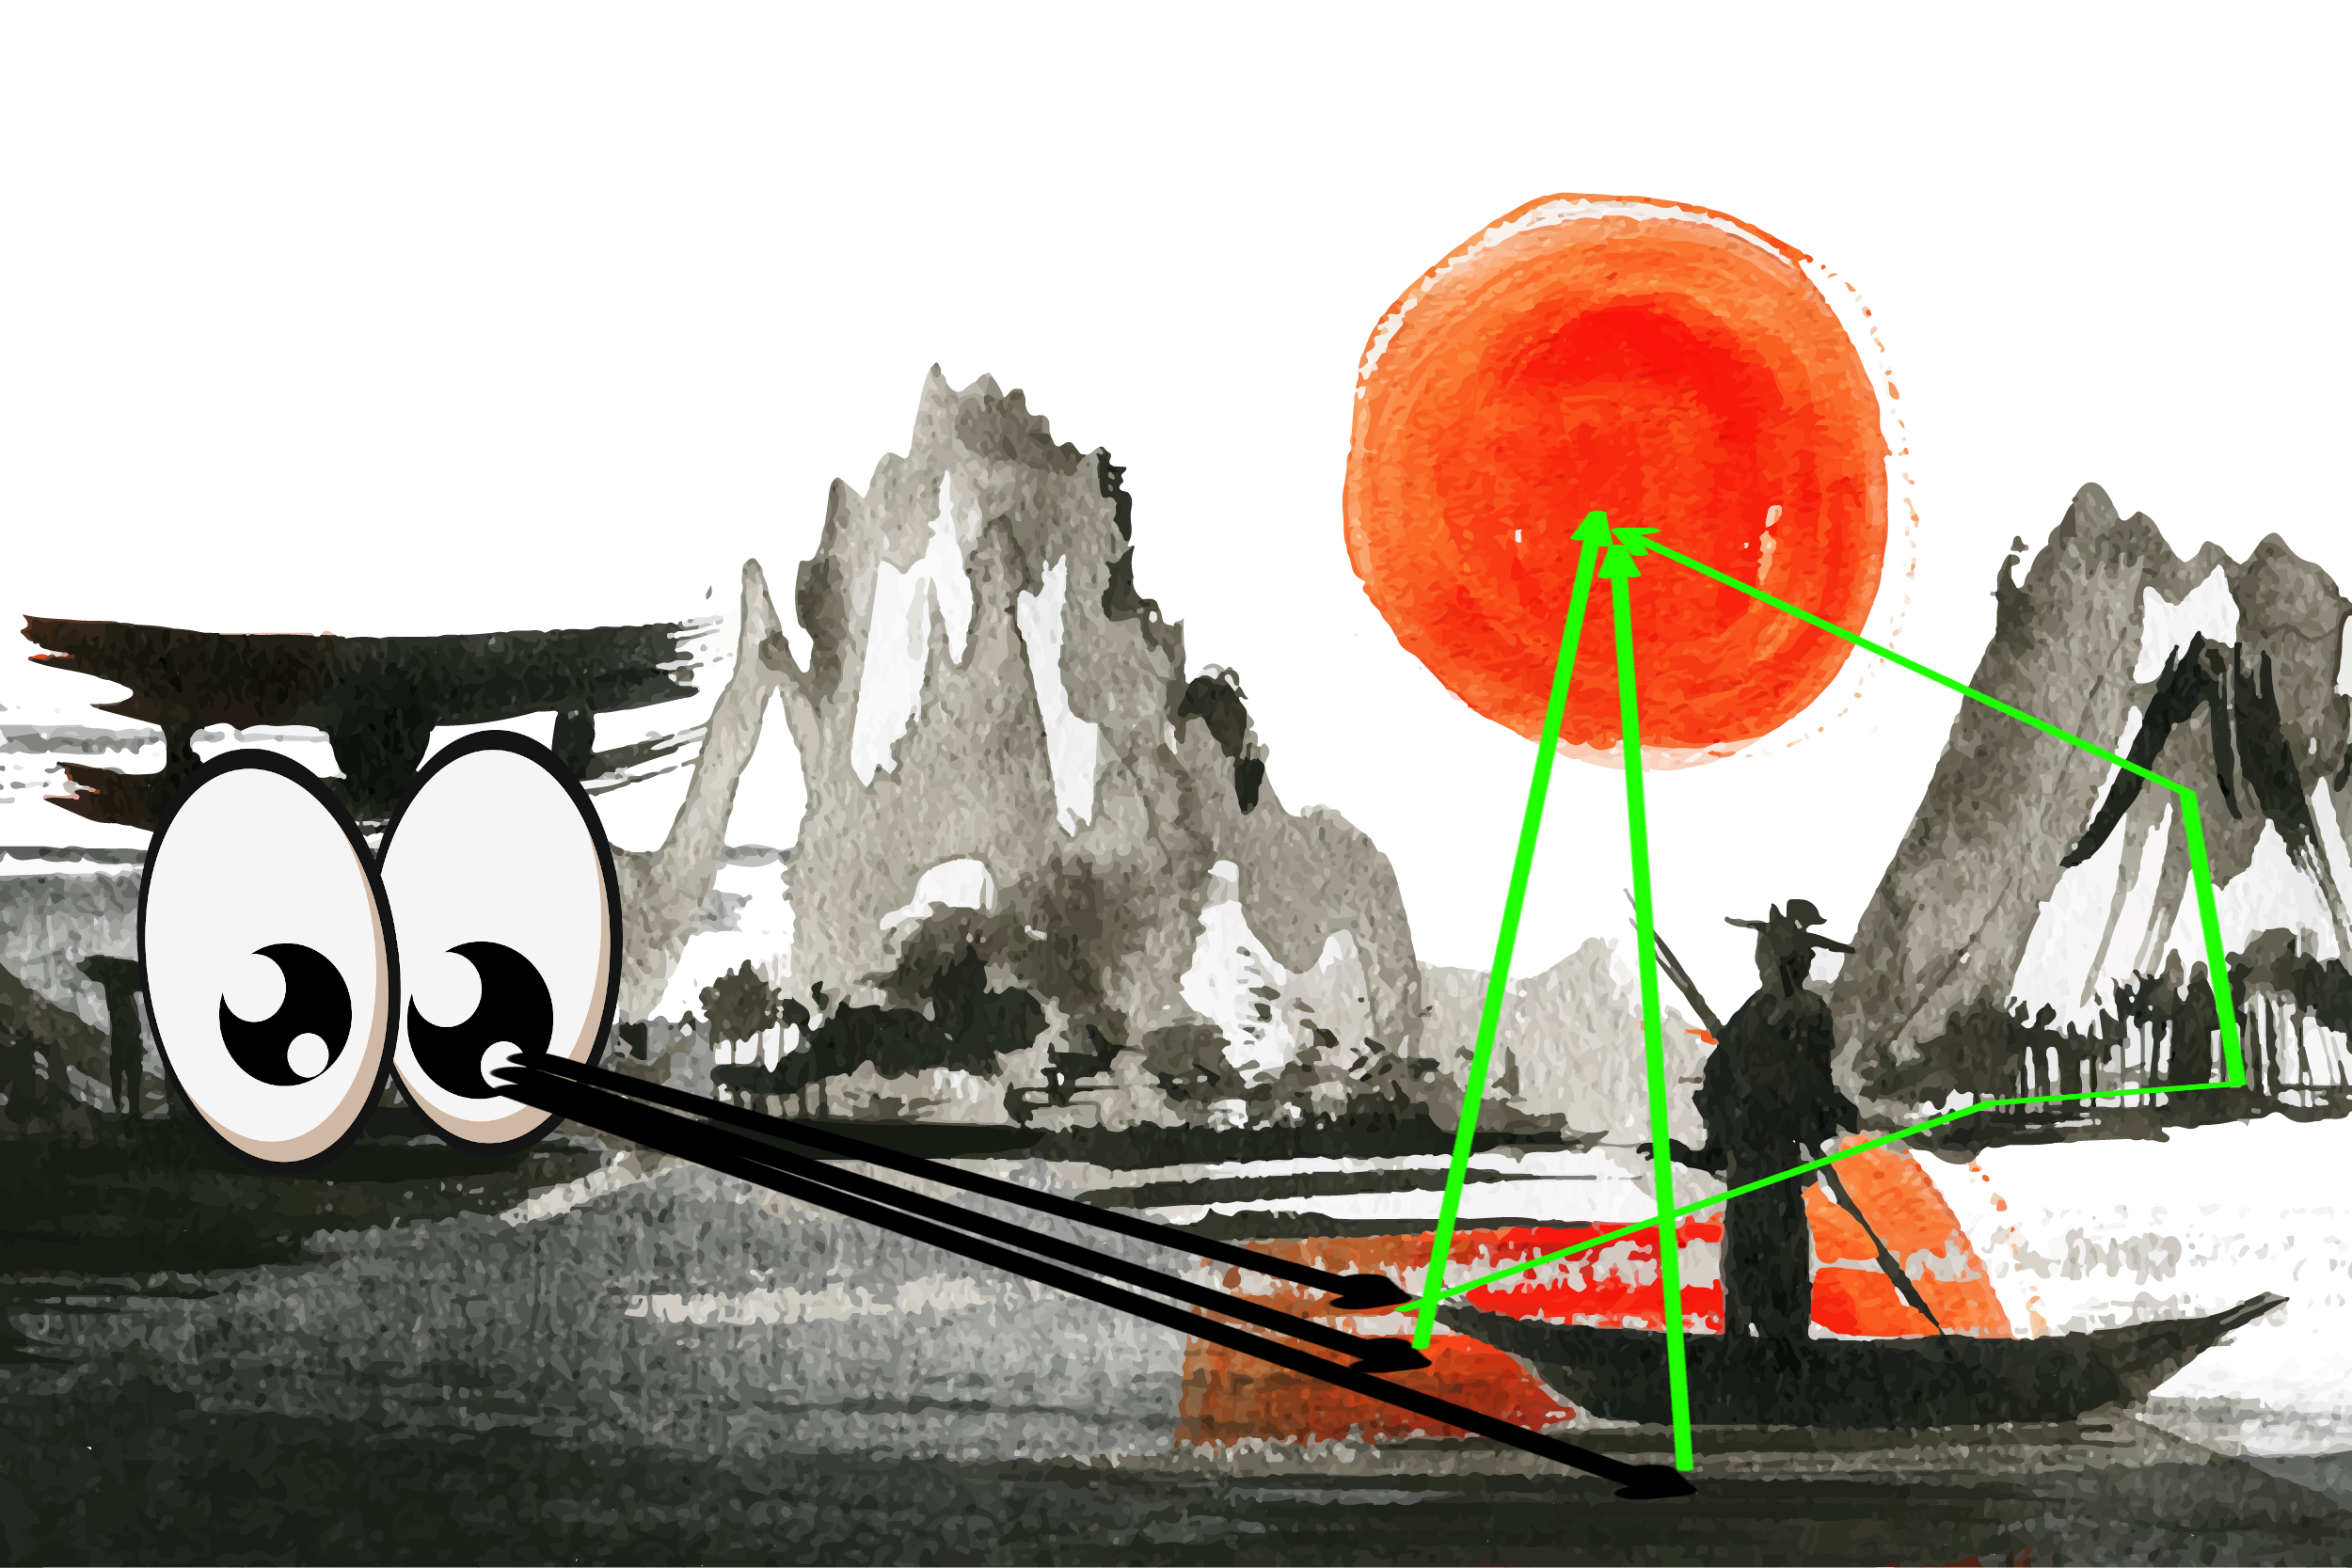
\includegraphics[width=\linewidth]{content/PathTracer/Bilder/PathTracerGuide.png}
    \caption{Grundkonzept Strahlverfolgung}
    \label{pic::GrundkonzeptPathTracing}
\end{figure}

Klassischerweiße werden hierbei pro Pixel mehrere zufällige Strahlen verschossen, welche jeder 
für sich einen \textit{Samplewert} ergibt und zur Farbgebung des Pixels beiträgt. Mehrere
unkorrelierte zufällige Folgen ergeben somit die schlussendliche Pixelfarbe. Der Fehler, der 
bei der zugrundeliegenden Monte-Carlo Integration (siehe Gleichung \ref{eq:Monte-Carlo}) entsteht, 
wird klassischerweiße 
über Varianzreduktionsmethoden (minimiere Gleichung \ref{eq:Monte-Carlo-Varianz}) wie \textit{Importance Sampling}
angegangen.
Das Ziel hierbei ist es, die Fehlerverteilung im Bildraum zu beeinflussen, da diese für die wahrnehmbare 
visuelle Qualität des Bildes verantwortlich ist. Diese Arbeit wird vom diesen Vorgehen abweichen und direkt im 
Bildraum eine zeitlich stabile \nameref{ch:Content1:sec:blue noise}
Fehlerverteilung durch korrelierte Folgen erreichen. Die positive Auswirkung von \nameref{ch:Content1:sec:blue noise} 
Verteilungen auf die visuelle Qualität wurde bereits ausgiebig erforscht \cite{3288}.

\par 

Der \nameref{ch:Content1:sec:Path Tracer} ist in Hinsicht der Beleuchtung komplett. 
Deshalb verwenden wir den \nameref{ch:Content1:sec:Path Tracer} um innerhalb unseren Render Graphen
(siehe Abbildung \ref{pic:Render Graph}) die \textit{Global Illumination} zu erreichen. 
Der hier verwendete \nameref{ch:Content1:sec:Path Tracer} wurde mit dem Framework umgesetzt und
(siehe \cite{Benty18}) beruht auf Erkenntnisse der Lösung der allgemeinen Rendergleichung
(siehe Gleichung \ref{eq:Allgemeine Rendergleichung}).

\begin{equation}\label{eq:Allgemeine Rendergleichung}
    I(x,{x}^{'}) = g(x,{x}^{'}) * \biggl[\epsilon(x,{x}^{'}) + 
    \int_{S}^{} \rho(x,{x}^{'},{x}^{''})
    I({x}^{'},{x}^{''}d{x}^{''})\biggr] 
\end{equation}

Sie beschreibt den Energietransport \textit{I} von einem Punkt ${x}^{'}$
zu einem Punkt x. Dabei ist ein maßgebender Faktor der Geometrieterm \textit{g},
der die relative Lage der beiden Punkte zueinander im Raum beschreibt.
Ein weiterer Faktor ist die Abstrahlung \textit{$\epsilon$} von ${x}^{'}$ nach x. 
Beeinflusst wird der Energiefluss auch durch
die bidirektionale Verteilungsfunktion \textit{$\rho$}, welche Aufschluss über
das einfallende Licht von einem Punkt ${x}^{''}$ über ${x}^{'}$ zu x gibt.\par
Die Schlussfolgerung aus dieser Gleichung \ref{eq:Allgemeine Rendergleichung} ist: Die transportierte
Intensität von einem Punkt zu einem Anderen ist die Summe des ausgestrahlten Lichts 
und das reflektierte Licht zu x von allen anderen Oberflächen x.

Ausgehend von der Rendergleichung \ref{eq:Allgemeine Rendergleichung} lässt sich
die vollständige Transportgleichung \ref{eq:vollständige Transportgleichung}
beschreiben.
Wie von \cite{marschner2009fundamentals} beschrieben wird ausgehend von der vollständigen Transportgleichung
\nameref{eq:vollständige Transportgleichung}

\begin{equation}\label{eq:vollständige Transportgleichung}
    L_s(k_0) = L_e(k_0) + \int_{all(k_i)}^{} \rho(k_i, k_0)*L_f(k_i)*cos(\theta_i)d\theta_i
\end{equation}

der vollständige Lichttransport beschrieben. Man kann deutlich die Ähnlichkeit
zu \nameref{eq:Allgemeine Rendergleichung} erkennen. Wir haben den Emissionsterm, die relative Lage der 
Punkte zueinander und die bidirektionale Verteilungsfunktion welche den Energietransport
beeinflussen.


\subsubsection{Monte-Carlo-Integration}
Mit der Monte Carlo Integration approximieren wir die Rendergleichung.\ref{eq:Allgemeine Rendergleichung} 
Bei gegebener Dimensionalität n des Renderintegrals und der 
Wahrscheinlichkeitsdichtefunktion $\rho(x_i)$
(siehe auch \cite{KK02})

\begin{equation}\label{eq:Monte-Carlo}
    E\biggl[\frac{1}{k}\sum_{i=1}^{k}\frac{f(X_{i})}{\rho(X_{i})}\biggl] = \int_{[0,1]^{n}}f(x)dx
\end{equation}

Dabei wird das n-dimensionale Integral \ref{eq:vollständige Transportgleichung} approximiert. Die Dichtefunktion $\rho(x_i)$ 
deutet an, dass hierbei die Stichproben auch nicht-uniform genommen werden können. 
Varianzreduktionsmethoden machen sich diese Dichtefunktion zu Nutze um 
ein besseres Ergebnis zu bekommen (nach \cite{caflisch_1998}).
Die Konvergenzrate ist unabhängig von der Dimension unseres \nameref{ch:Content1:sec:Path Tracer}
\textit{O}($N^{-\frac{1}{2}}$) und ist robust, das heißt Exaktheit hängt nur vom ungenauesten Parameter ab.
Eine Variante des Verfahrens, die Monte Carlo Quadratur, wird mit quasi zufälligen Sequenzen \nameref{ch:Content1:sec:Quasi-Zufallsfolgen}, 
welche eine niedrige Abweichung aufweisen, durchgeführt.
Um die Konvergenzrate zu steigern liegen eine Reihe von Varianzreduktionsmethoden vor. Jedoch werden wird hier 
einen Temporalen Algorithmus (siehe Kapitel \ref{ch:Temporaler Algorithmus}) anwenden und damit eine direkte Umverteilung im Bildraum 
umsetzen.

\begin{equation}\label{eq:Monte-Carlo-Varianz}
    V[X] = E\biggl[(X-E[X])^{2}\biggl] = E[X^{2}]
    - E[X]^{2}
\end{equation}

\subsubsection{DirectX Raytracing}

\begin{figure}[H]
    \centering
    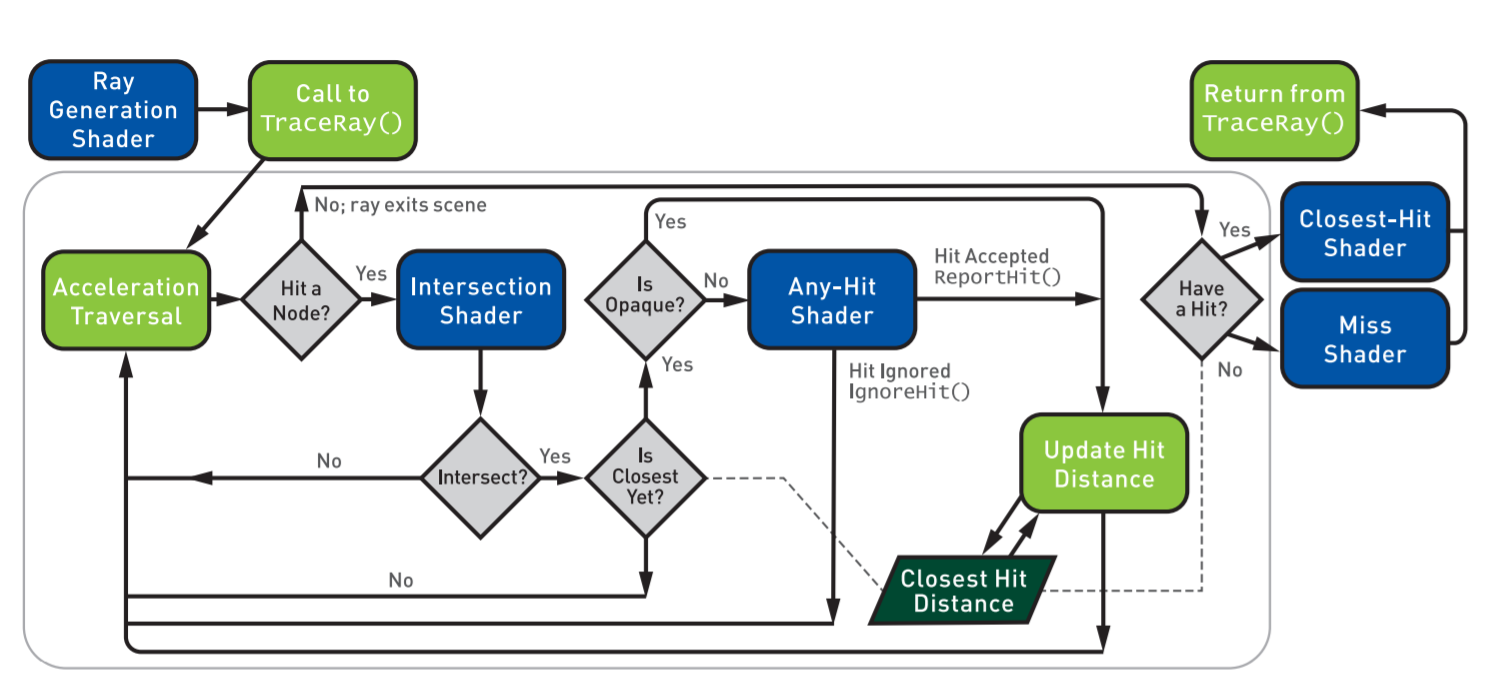
\includegraphics[width=\linewidth]{content/PathTracer/Bilder/DirectXRaytracingPipeline.png}
    \caption{DirectX Raytracing Pipeline aus \cite{Haines2019}}
    \label{pic:DirectXRaytracingPipeline}
\end{figure}

Das hardwareunterstützte Raytracing erhielt Einzug in moderne Programmierschnittstellen(DirectX, Vulkan) und wird 
hier anhand von DirectX erläutert, welche auch für die \textit{Global Illumination} innerhalb des 
Render Graphs \ref{pic:Render Graph} benutzt wurde. 

Im Folgenden Algorithmus \ref{alg:Path Tracer Konzept} wird nochmal vereinfacht die Funktionsweise 
eines Path Tracers erläutert, wobei die entsprechenden programmierbaren Shader von DirectX 
im jeweiligen Codeabschnitt markiert sind.

\begin{algorithm}[H]
    \caption{Path Tracing Algorithmus}
    \begin{algorithmic}[1]
        \Procedure{Trace Path}{$BVH$}\Comment{verfolge Pfad durch Szene}
        \For{(x,y) $\in$ frame}
        \State strahl = verschiesseStrahlInPixel(x,y); // \textbf{ray generation shader}
        \For{blatt = bekommeBVHBlatt()}
        \State schnittpunkt = schneideGeometrie(strahl, blatt); //\textbf{Intersection shader}
        \If{schnittpunkt $\leq$ nähesterSchnittpunkt}
        \State aktualisiereNähestenSchnittpunkt();
        \EndIf
        \EndFor
        \If{Schnittpunkt gefunden}
        \State frame(x,y) = gebeFarbe(strahl,nähesterSchnittpunkt); //\textbf{closest-hit shader}
        \Else
        \State frame(x,y) = Umgebungskarte(x,y);//\textbf{miss shader}
        \EndIf
        \EndFor
        \EndProcedure
    \end{algorithmic}
    \label{alg:Path Tracer Konzept}
\end{algorithm}


In Abbildung \ref{pic:DirectXRaytracingPipeline} und  Algorithmus \ref{alg:Path Tracer Konzept} lässt sich
der Beginn (Generierung eines Strahles) der neuen Pipeline durch den programmierbaren
\textbf{Ray Generation shader} erkennen.

\begin{algorithm}[H]
    \caption{Beispielhafter minimalistischer Ray Generation Shader}
    \begin{algorithmic}[1]
        \State [shader(\dq raygeneration \dq)]
        \State launchIndex = DispatchRaysIndex().xy;
        \For{(int i = 0; i < numberOfRays;i++)}
            \State float shadowRayMult = TraceRay(gRtScene,
            RAY\_FLAG\_ACCEPT\_FIRST\_HIT \_AND\_END\_SEARCH |
            RAY\_FLAG\_SKIP\_CLOSEST\_HIT\_SHADER,
            0xFF, 0, hitProgramCount, 0, ray, payload);
            \State float indirectRayColor = TraceRay(gRtScene, 0, 0xFF, 1, hitProgramCount, 1, rayColor, payload);
            \State color = shadowRayMult * shadingColor + computeindirectLighting(indirectRayColor);
        \EndFor
        \State output[id] = color;
    \end{algorithmic}
    \label{alg:Ray Gen}
\end{algorithm}

Mit Hilfe der Methode \textbf{TraceRay()} werden dann zur Beleuchtungsberechnung 
die Strahlen verschossen. Damit diese Methode richtig arbeiten kann übergeben wir neben unseren Strahl 
unter Anderem  unsere Szene inklusive Beschleunigungsstruktur, rayflags 
(beeinflussen Transparaenz, Culling, Abbruch)\cite{RayFlags} und einen payload.
Mit dem \textit{$payload_t$} können wir einen struct mit Informationen jedem einzelnen Strahl mitgeben.

\begin{algorithm}[H]
    \caption{beispielhafter payload}
    \begin{algorithmic}[1]
        \State struct RayPayload = {float4 color, uint32 seed, uint32 depth};        
        \end{algorithmic}
        \label{alg:payload}
    \end{algorithm}
    
Diese Methode \textbf{TraceRay()} kann auch innerhalb der anderen Shader zum weiteren verschießen
von Strahlen verwendet werden. So beispielweise beim Verschießen eines Schattenstrahls mit flags 
RAY\_FLAG\_ACCEPT\_FIRST\_HIT\_AND\_END\_SEARCH, \newline
RAY\_FLAG\_SKIP\_CLOSEST\_HIT\_SHADER setzen, um unnötige 
Beleuchtungsberechnungen und weitere Schnittpunktberechnungen zu umgehen und mit einem Bit als payload 
die Sichtbarkeit zur Lichtquelle mitzugeben.
Mit diesem beispielhaften payload können wir die Farbe akkumulieren, unsere  
seeds verwenden um z.B eine weiteren Strahlenschuss in einem Any-Hit Shader zu verwirklichen,  
solange die mit übergebene Rekursionstiefe in unserem payload eingehalten wird.  

\textbf{Intersection shader} führt die Schnittberechnungen durch.
Haben wir eine Szene, welche aus ausschließlich Dreiecken besteht, können wir
die auf Hardware standardmäßig gelieferte Implementierung übernehmen. 
Optionale Berechnungen für andere Geometrie können hier implementiert werden.
Bei einem gefundenen nähsten Schnittpunkt einer durchsichtigen Oberfläche wird der 
\textit{Any-hit shader} aufgerufen.
\textbf{Any-hit shaders} erlauben klassische \textit{Discards} oder informieren
über einen korrekten Schnitt. So können wir z.B. einen Alpha Test durchführen.

\begin{algorithm}[H]
    \caption{Any-Hit shader}
    \begin{algorithmic}[1]
        \State [shader(\dq anyhit \dq)]
        \If{(!alphaTest)} 
        \State IgnoreHit();
        \EndIf
    \end{algorithmic}
    \label{alg:any hit}
\end{algorithm}

Der \textbf{Closest-hit shader} berechnet den Schnittpunkt des Strahls mit der Geometrie
der Szene, die dem Strahlursprung am nähesten ist.
Mit der Kennzeichnung [shader(\dq closesthit \dq)] wird die Hauptmethode zur 
dessen Ausführung markiert. An dieser Stelle bietet es sich an die Shading Farbe 
mit der Schnittpunktinformation zu aktualisieren und/oder um eine Rekursionstiefe weiter 
zu gehen einen weiteren Strahl zu verschießen. 
Der \textbf{miss shader} wird immer dann ausgeführt, wenn ein Strahl die
Szenengeometrie nicht schneidet. Kann also für das Nachschauen in einer 
Environment Map verwendet werden. 

\subsection{Render Graph}

\begin{figure}[H]
    \centering
    \def\svgwidth{\columnwidth}
    \import{content/PathTracer/Bilder/}{render_graph.pdf_tex}
    \caption{Unser Render Graph}
    \label{pic:Render Graph}
\end{figure}






